\documentclass[1p]{elsarticle_modified}
%\bibliographystyle{elsarticle-num}

%\usepackage[colorlinks]{hyperref}
%\usepackage{abbrmath_seonhwa} %\Abb, \Ascr, \Acal ,\Abf, \Afrak
\usepackage{amsfonts}
\usepackage{amssymb}
\usepackage{amsmath}
\usepackage{amsthm}
\usepackage{scalefnt}
\usepackage{amsbsy}
\usepackage{kotex}
\usepackage{caption}
\usepackage{subfig}
\usepackage{color}
\usepackage{graphicx}
\usepackage{xcolor} %% white, black, red, green, blue, cyan, magenta, yellow
\usepackage{float}
\usepackage{setspace}
\usepackage{hyperref}

\usepackage{tikz}
\usetikzlibrary{arrows}

\usepackage{multirow}
\usepackage{array} % fixed length table
\usepackage{hhline}

%%%%%%%%%%%%%%%%%%%%%
\makeatletter
\renewcommand*\env@matrix[1][\arraystretch]{%
	\edef\arraystretch{#1}%
	\hskip -\arraycolsep
	\let\@ifnextchar\new@ifnextchar
	\array{*\c@MaxMatrixCols c}}
\makeatother %https://tex.stackexchange.com/questions/14071/how-can-i-increase-the-line-spacing-in-a-matrix
%%%%%%%%%%%%%%%

\usepackage[normalem]{ulem}

\newcommand{\msout}[1]{\ifmmode\text{\sout{\ensuremath{#1}}}\else\sout{#1}\fi}
%SOURCE: \msout is \stkout macro in https://tex.stackexchange.com/questions/20609/strikeout-in-math-mode

\newcommand{\cancel}[1]{
	\ifmmode
	{\color{red}\msout{#1}}
	\else
	{\color{red}\sout{#1}}
	\fi
}

\newcommand{\add}[1]{
	{\color{blue}\uwave{#1}}
}

\newcommand{\replace}[2]{
	\ifmmode
	{\color{red}\msout{#1}}{\color{blue}\uwave{#2}}
	\else
	{\color{red}\sout{#1}}{\color{blue}\uwave{#2}}
	\fi
}

\newcommand{\Sol}{\mathcal{S}} %segment
\newcommand{\D}{D} %diagram
\newcommand{\A}{\mathcal{A}} %arc


%%%%%%%%%%%%%%%%%%%%%%%%%%%%%5 test

\def\sl{\operatorname{\textup{SL}}(2,\Cbb)}
\def\psl{\operatorname{\textup{PSL}}(2,\Cbb)}
\def\quan{\mkern 1mu \triangleright \mkern 1mu}

\theoremstyle{definition}
\newtheorem{thm}{Theorem}[section]
\newtheorem{prop}[thm]{Proposition}
\newtheorem{lem}[thm]{Lemma}
\newtheorem{ques}[thm]{Question}
\newtheorem{cor}[thm]{Corollary}
\newtheorem{defn}[thm]{Definition}
\newtheorem{exam}[thm]{Example}
\newtheorem{rmk}[thm]{Remark}
\newtheorem{alg}[thm]{Algorithm}

\newcommand{\I}{\sqrt{-1}}
\begin{document}

%\begin{frontmatter}
%
%\title{Boundary parabolic representations of knots up to 8 crossings}
%
%%% Group authors per affiliation:
%\author{Yunhi Cho} 
%\address{Department of Mathematics, University of Seoul, Seoul, Korea}
%\ead{yhcho@uos.ac.kr}
%
%
%\author{Seonhwa Kim} %\fnref{s_kim}}
%\address{Center for Geometry and Physics, Institute for Basic Science, Pohang, 37673, Korea}
%\ead{ryeona17@ibs.re.kr}
%
%\author{Hyuk Kim}
%\address{Department of Mathematical Sciences, Seoul National University, Seoul 08826, Korea}
%\ead{hyukkim@snu.ac.kr}
%
%\author{Seokbeom Yoon}
%\address{Department of Mathematical Sciences, Seoul National University, Seoul, 08826,  Korea}
%\ead{sbyoon15@snu.ac.kr}
%
%\begin{abstract}
%We find all boundary parabolic representation of knots up to 8 crossings.
%
%\end{abstract}
%\begin{keyword}
%    \MSC[2010] 57M25 
%\end{keyword}
%
%\end{frontmatter}

%\linenumbers
%\tableofcontents
%
\newcommand\colored[1]{\textcolor{white}{\rule[-0.35ex]{0.8em}{1.4ex}}\kern-0.8em\color{red} #1}%
%\newcommand\colored[1]{\textcolor{white}{ #1}\kern-2.17ex	\textcolor{white}{ #1}\kern-1.81ex	\textcolor{white}{ #1}\kern-2.15ex\color{red}#1	}

{\Large $\underline{12a_{0501}~(K12a_{0501})}$}

\setlength{\tabcolsep}{10pt}
\renewcommand{\arraystretch}{1.6}
\vspace{1cm}\begin{tabular}{m{100pt}>{\centering\arraybackslash}m{274pt}}
\multirow{5}{120pt}{
	\centering
	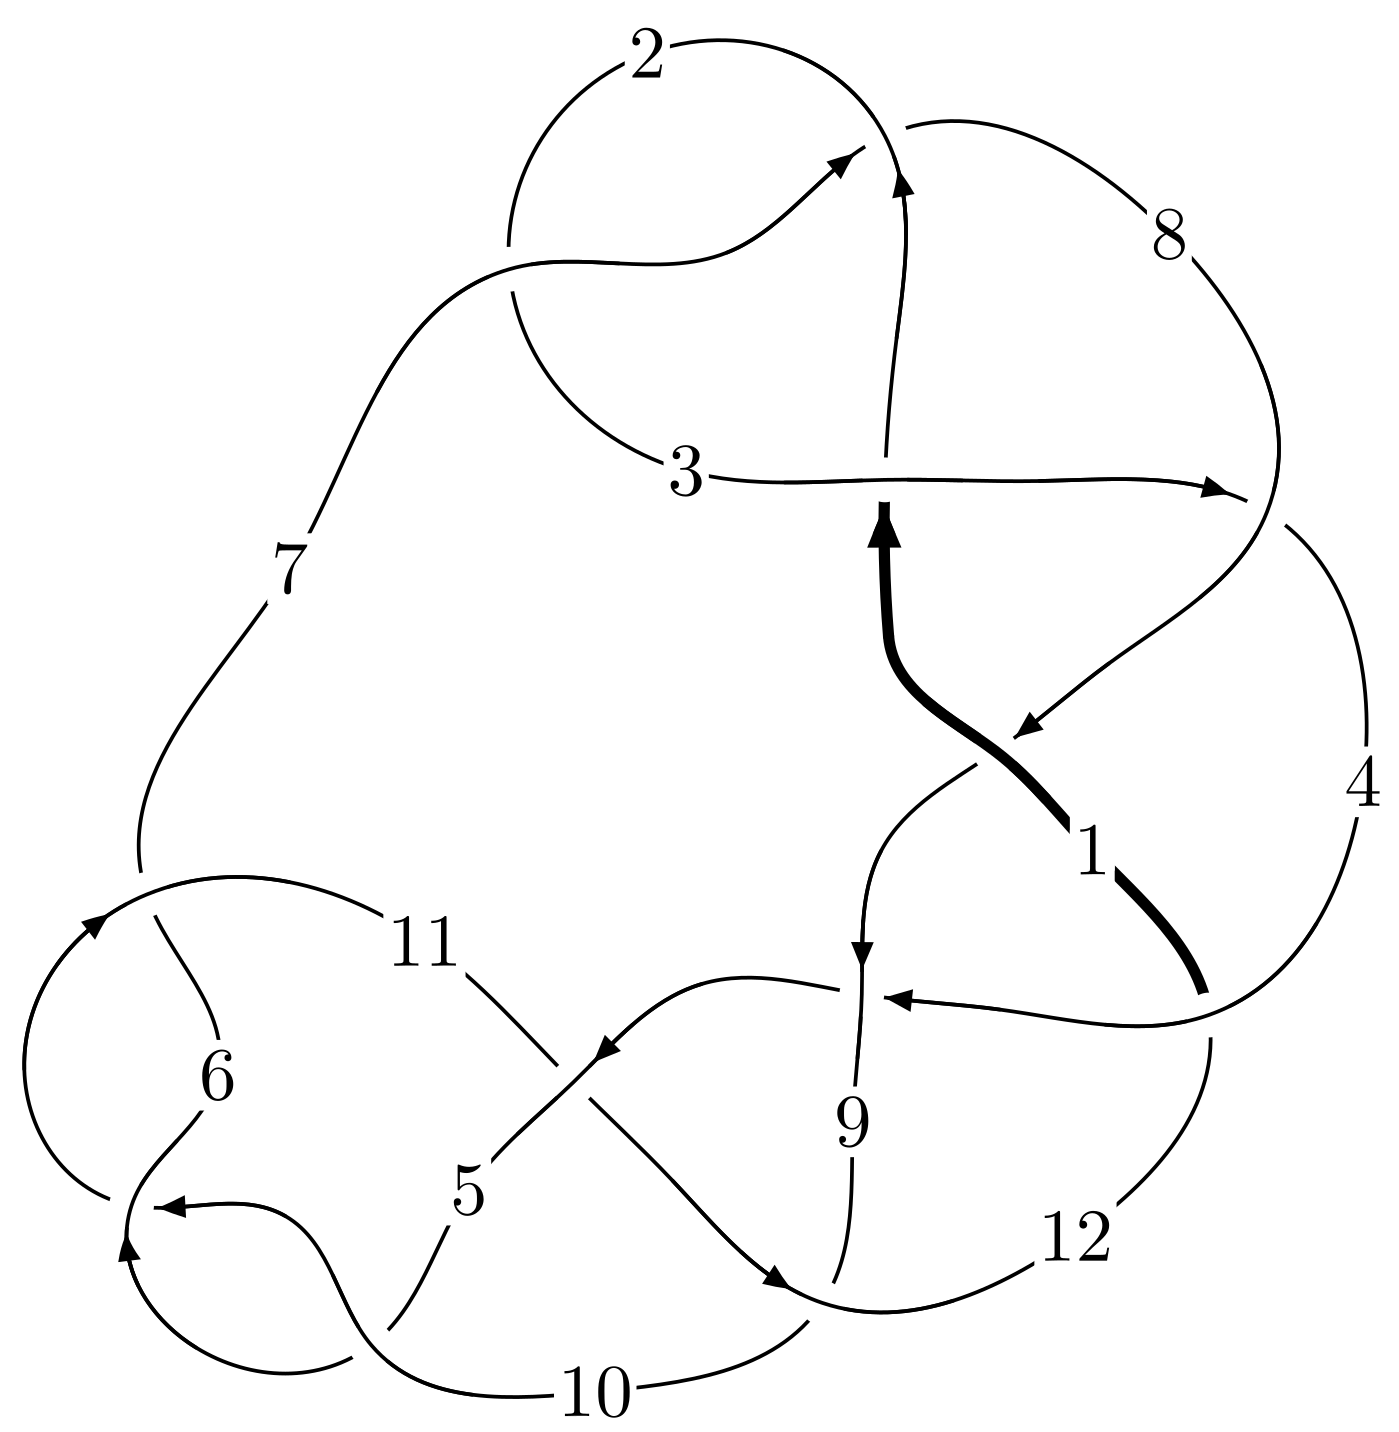
\includegraphics[width=112pt]{../../../GIT/diagram.site/Diagrams/png/1302_12a_0501.png}\\
\ \ \ A knot diagram\footnotemark}&
\allowdisplaybreaks
\textbf{Linearized knot diagam} \\
\cline{2-2}
 &
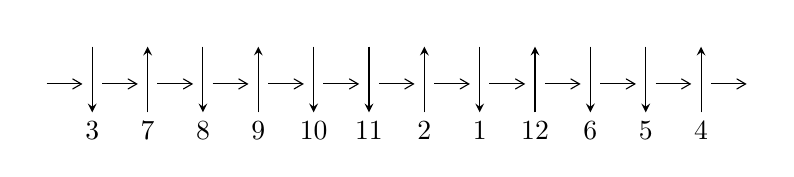
\begin{tikzpicture}[x=20pt, y=17pt]
	% nodes
	\node (C0) at (0, 0) {};
	\node (C1) at (1, 0) {};
	\node (C1U) at (1, +1) {};
	\node (C1D) at (1, -1) {3};

	\node (C2) at (2, 0) {};
	\node (C2U) at (2, +1) {};
	\node (C2D) at (2, -1) {7};

	\node (C3) at (3, 0) {};
	\node (C3U) at (3, +1) {};
	\node (C3D) at (3, -1) {8};

	\node (C4) at (4, 0) {};
	\node (C4U) at (4, +1) {};
	\node (C4D) at (4, -1) {9};

	\node (C5) at (5, 0) {};
	\node (C5U) at (5, +1) {};
	\node (C5D) at (5, -1) {10};

	\node (C6) at (6, 0) {};
	\node (C6U) at (6, +1) {};
	\node (C6D) at (6, -1) {11};

	\node (C7) at (7, 0) {};
	\node (C7U) at (7, +1) {};
	\node (C7D) at (7, -1) {2};

	\node (C8) at (8, 0) {};
	\node (C8U) at (8, +1) {};
	\node (C8D) at (8, -1) {1};

	\node (C9) at (9, 0) {};
	\node (C9U) at (9, +1) {};
	\node (C9D) at (9, -1) {12};

	\node (C10) at (10, 0) {};
	\node (C10U) at (10, +1) {};
	\node (C10D) at (10, -1) {6};

	\node (C11) at (11, 0) {};
	\node (C11U) at (11, +1) {};
	\node (C11D) at (11, -1) {5};

	\node (C12) at (12, 0) {};
	\node (C12U) at (12, +1) {};
	\node (C12D) at (12, -1) {4};
	\node (C13) at (13, 0) {};

	% arrows
	\draw[->,>={angle 60}]
	(C0) edge (C1) (C1) edge (C2) (C2) edge (C3) (C3) edge (C4) (C4) edge (C5) (C5) edge (C6) (C6) edge (C7) (C7) edge (C8) (C8) edge (C9) (C9) edge (C10) (C10) edge (C11) (C11) edge (C12) (C12) edge (C13) ;	\draw[->,>=stealth]
	(C1U) edge (C1D) (C2D) edge (C2U) (C3U) edge (C3D) (C4D) edge (C4U) (C5U) edge (C5D) (C6U) edge (C6D) (C7D) edge (C7U) (C8U) edge (C8D) (C9D) edge (C9U) (C10U) edge (C10D) (C11U) edge (C11D) (C12D) edge (C12U) ;
	\end{tikzpicture} \\
\hhline{~~} \\& 
\textbf{Solving Sequence} \\ \cline{2-2} 
 &
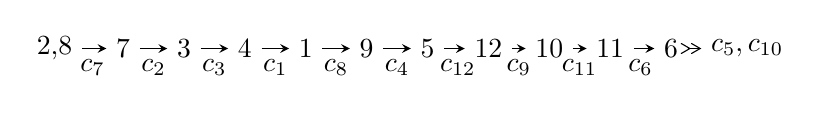
\begin{tikzpicture}[x=22pt, y=7pt]
	% node
	\node (A0) at (-1/8, 0) {2,8};
	\node (A1) at (1, 0) {7};
	\node (A2) at (2, 0) {3};
	\node (A3) at (3, 0) {4};
	\node (A4) at (4, 0) {1};
	\node (A5) at (5, 0) {9};
	\node (A6) at (6, 0) {5};
	\node (A7) at (7, 0) {12};
	\node (A8) at (8, 0) {10};
	\node (A9) at (9, 0) {11};
	\node (A10) at (10, 0) {6};
	\node (C1) at (1/2, -1) {$c_{7}$};
	\node (C2) at (3/2, -1) {$c_{2}$};
	\node (C3) at (5/2, -1) {$c_{3}$};
	\node (C4) at (7/2, -1) {$c_{1}$};
	\node (C5) at (9/2, -1) {$c_{8}$};
	\node (C6) at (11/2, -1) {$c_{4}$};
	\node (C7) at (13/2, -1) {$c_{12}$};
	\node (C8) at (15/2, -1) {$c_{9}$};
	\node (C9) at (17/2, -1) {$c_{11}$};
	\node (C10) at (19/2, -1) {$c_{6}$};
	\node (A11) at (45/4, 0) {$c_{5},c_{10}$};

	% edge
	\draw[->,>=stealth]	
	(A0) edge (A1) (A1) edge (A2) (A2) edge (A3) (A3) edge (A4) (A4) edge (A5) (A5) edge (A6) (A6) edge (A7) (A7) edge (A8) (A8) edge (A9) (A9) edge (A10) ;
	\draw[->>,>={angle 60}]	
	(A10) edge (A11);
\end{tikzpicture} \\ 

\end{tabular} \\

\footnotetext{
The image of knot diagram is generated by the software ``\textbf{Draw programme}" developed by Andrew Bartholomew(\url{http://www.layer8.co.uk/maths/draw/index.htm\#Running-draw}), where we modified some parts for our purpose(\url{https://github.com/CATsTAILs/LinksPainter}).
}\phantom \\ \newline 
\centering \textbf{Ideals for irreducible components\footnotemark of $X_{\text{par}}$} 
 
\begin{align*}
I^u_{1}&=\langle 
u^{99}+u^{98}+\cdots+2 u+1\rangle \\
\\
\end{align*}
\raggedright * 1 irreducible components of $\dim_{\mathbb{C}}=0$, with total 99 representations.\\
\footnotetext{All coefficients of polynomials are rational numbers. But the coefficients are sometimes approximated in decimal forms when there is not enough margin.}
\newpage
\renewcommand{\arraystretch}{1}
\centering \section*{I. $I^u_{1}= \langle u^{99}+u^{98}+\cdots+2 u+1 \rangle$}
\flushleft \textbf{(i) Arc colorings}\\
\begin{tabular}{m{7pt} m{180pt} m{7pt} m{180pt} }
\flushright $a_{2}=$&$\begin{pmatrix}0\\u\end{pmatrix}$ \\
\flushright $a_{8}=$&$\begin{pmatrix}1\\0\end{pmatrix}$ \\
\flushright $a_{7}=$&$\begin{pmatrix}1\\u^2\end{pmatrix}$ \\
\flushright $a_{3}=$&$\begin{pmatrix}u\\u^3+u\end{pmatrix}$ \\
\flushright $a_{4}=$&$\begin{pmatrix}- u^3\\u^3+u\end{pmatrix}$ \\
\flushright $a_{1}=$&$\begin{pmatrix}u^3\\u^5+u^3+u\end{pmatrix}$ \\
\flushright $a_{9}=$&$\begin{pmatrix}u^8+u^6+u^4+1\\u^{10}+2 u^8+3 u^6+2 u^4+u^2\end{pmatrix}$ \\
\flushright $a_{5}=$&$\begin{pmatrix}u^{21}+4 u^{19}+9 u^{17}+12 u^{15}+12 u^{13}+10 u^{11}+9 u^9+6 u^7+3 u^5+u\\u^{23}+5 u^{21}+\cdots+2 u^3+u\end{pmatrix}$ \\
\flushright $a_{12}=$&$\begin{pmatrix}- u^{11}-2 u^9-2 u^7+u^3\\u^{11}+3 u^9+4 u^7+3 u^5+u^3+u\end{pmatrix}$ \\
\flushright $a_{10}=$&$\begin{pmatrix}u^{32}+7 u^{30}+\cdots+2 u^{12}+1\\- u^{32}-8 u^{30}+\cdots-12 u^8-4 u^6\end{pmatrix}$ \\
\flushright $a_{11}=$&$\begin{pmatrix}u^{55}+12 u^{53}+\cdots+5 u^7+2 u^3\\u^{57}+13 u^{55}+\cdots+2 u^3+u\end{pmatrix}$ \\
\flushright $a_{6}=$&$\begin{pmatrix}- u^{87}-20 u^{85}+\cdots-5 u^7-2 u^3\\u^{87}+21 u^{85}+\cdots+2 u^3+u\end{pmatrix}$\\&\end{tabular}
\flushleft \textbf{(ii) Obstruction class $= -1$}\\~\\
\flushleft \textbf{(iii) Cusp Shapes $= -4 u^{97}-4 u^{96}+\cdots-12 u-10$}\\~\\
\newpage\renewcommand{\arraystretch}{1}
\flushleft \textbf{(iv) u-Polynomials at the component}\newline \\
\begin{tabular}{m{50pt}|m{274pt}}
Crossings & \hspace{64pt}u-Polynomials at each crossing \\
\hline $$\begin{aligned}c_{1}\end{aligned}$$&$\begin{aligned}
&u^{99}+47 u^{98}+\cdots-2 u-1
\end{aligned}$\\
\hline $$\begin{aligned}c_{2},c_{7}\end{aligned}$$&$\begin{aligned}
&u^{99}+u^{98}+\cdots+2 u+1
\end{aligned}$\\
\hline $$\begin{aligned}c_{3}\end{aligned}$$&$\begin{aligned}
&u^{99}- u^{98}+\cdots-2396 u+457
\end{aligned}$\\
\hline $$\begin{aligned}c_{4}\end{aligned}$$&$\begin{aligned}
&u^{99}+u^{98}+\cdots-1366 u+521
\end{aligned}$\\
\hline $$\begin{aligned}c_{5},c_{6},c_{10}\end{aligned}$$&$\begin{aligned}
&u^{99}- u^{98}+\cdots+2 u+1
\end{aligned}$\\
\hline $$\begin{aligned}c_{8}\end{aligned}$$&$\begin{aligned}
&u^{99}+5 u^{98}+\cdots+1102 u+57
\end{aligned}$\\
\hline $$\begin{aligned}c_{9}\end{aligned}$$&$\begin{aligned}
&u^{99}+21 u^{98}+\cdots+218716 u+11327
\end{aligned}$\\
\hline $$\begin{aligned}c_{11}\end{aligned}$$&$\begin{aligned}
&u^{99}+3 u^{98}+\cdots-14 u-3
\end{aligned}$\\
\hline $$\begin{aligned}c_{12}\end{aligned}$$&$\begin{aligned}
&u^{99}+11 u^{98}+\cdots+14402 u+701
\end{aligned}$\\
\hline
\end{tabular}\\~\\
\newpage\renewcommand{\arraystretch}{1}
\flushleft \textbf{(v) Riley Polynomials at the component}\newline \\
\begin{tabular}{m{50pt}|m{274pt}}
Crossings & \hspace{64pt}Riley Polynomials at each crossing \\
\hline $$\begin{aligned}c_{1}\end{aligned}$$&$\begin{aligned}
&y^{99}+11 y^{98}+\cdots+2 y-1
\end{aligned}$\\
\hline $$\begin{aligned}c_{2},c_{7}\end{aligned}$$&$\begin{aligned}
&y^{99}+47 y^{98}+\cdots-2 y-1
\end{aligned}$\\
\hline $$\begin{aligned}c_{3}\end{aligned}$$&$\begin{aligned}
&y^{99}-25 y^{98}+\cdots+8147378 y-208849
\end{aligned}$\\
\hline $$\begin{aligned}c_{4}\end{aligned}$$&$\begin{aligned}
&y^{99}-17 y^{98}+\cdots+17086450 y-271441
\end{aligned}$\\
\hline $$\begin{aligned}c_{5},c_{6},c_{10}\end{aligned}$$&$\begin{aligned}
&y^{99}-89 y^{98}+\cdots-2 y-1
\end{aligned}$\\
\hline $$\begin{aligned}c_{8}\end{aligned}$$&$\begin{aligned}
&y^{99}+19 y^{98}+\cdots+191938 y-3249
\end{aligned}$\\
\hline $$\begin{aligned}c_{9}\end{aligned}$$&$\begin{aligned}
&y^{99}+31 y^{98}+\cdots-2952423990 y-128300929
\end{aligned}$\\
\hline $$\begin{aligned}c_{11}\end{aligned}$$&$\begin{aligned}
&y^{99}-5 y^{98}+\cdots-218 y-9
\end{aligned}$\\
\hline $$\begin{aligned}c_{12}\end{aligned}$$&$\begin{aligned}
&y^{99}+23 y^{98}+\cdots-14304490 y-491401
\end{aligned}$\\
\hline
\end{tabular}\\~\\
\newpage\flushleft \textbf{(vi) Complex Volumes and Cusp Shapes}
$$\begin{array}{c|c|c}  
\text{Solutions to }I^u_{1}& \I (\text{vol} + \sqrt{-1}CS) & \text{Cusp shape}\\
 \hline 
\begin{aligned}
u &= -0.469814 + 0.889386 I\end{aligned}
 & -5.15974 - 3.45007 I & \phantom{-0.000000 } 0 \\ \hline\begin{aligned}
u &= -0.469814 - 0.889386 I\end{aligned}
 & -5.15974 + 3.45007 I & \phantom{-0.000000 } 0 \\ \hline\begin{aligned}
u &= -0.148767 + 0.934892 I\end{aligned}
 & -5.20598 - 3.73864 I & \phantom{-0.000000 } 0 \\ \hline\begin{aligned}
u &= -0.148767 - 0.934892 I\end{aligned}
 & -5.20598 + 3.73864 I & \phantom{-0.000000 } 0 \\ \hline\begin{aligned}
u &= \phantom{-}0.242603 + 1.031670 I\end{aligned}
 & -0.575080 + 0.871667 I & \phantom{-0.000000 } 0 \\ \hline\begin{aligned}
u &= \phantom{-}0.242603 - 1.031670 I\end{aligned}
 & -0.575080 - 0.871667 I & \phantom{-0.000000 } 0 \\ \hline\begin{aligned}
u &= \phantom{-}0.650159 + 0.633663 I\end{aligned}
 & -2.28389 + 9.47082 I & \phantom{-0.000000 } 0. - 7.96667 I \\ \hline\begin{aligned}
u &= \phantom{-}0.650159 - 0.633663 I\end{aligned}
 & -2.28389 - 9.47082 I & \phantom{-0.000000 -}0. + 7.96667 I \\ \hline\begin{aligned}
u &= \phantom{-}0.567446 + 0.934324 I\end{aligned}
 & -3.16890 - 4.70879 I & \phantom{-0.000000 } 0 \\ \hline\begin{aligned}
u &= \phantom{-}0.567446 - 0.934324 I\end{aligned}
 & -3.16890 + 4.70879 I & \phantom{-0.000000 } 0 \\ \hline\begin{aligned}
u &= -0.561044 + 0.947080 I\end{aligned}
 & \phantom{-}2.13253 + 1.20620 I & \phantom{-0.000000 } 0 \\ \hline\begin{aligned}
u &= -0.561044 - 0.947080 I\end{aligned}
 & \phantom{-}2.13253 - 1.20620 I & \phantom{-0.000000 } 0 \\ \hline\begin{aligned}
u &= -0.645418 + 0.621535 I\end{aligned}
 & \phantom{-}3.08946 - 5.93342 I & \phantom{-}2.82989 + 7.73749 I \\ \hline\begin{aligned}
u &= -0.645418 - 0.621535 I\end{aligned}
 & \phantom{-}3.08946 + 5.93342 I & \phantom{-}2.82989 - 7.73749 I \\ \hline\begin{aligned}
u &= -0.226159 + 1.083640 I\end{aligned}
 & -3.58165 + 2.19221 I & \phantom{-0.000000 } 0 \\ \hline\begin{aligned}
u &= -0.226159 - 1.083640 I\end{aligned}
 & -3.58165 - 2.19221 I & \phantom{-0.000000 } 0 \\ \hline\begin{aligned}
u &= \phantom{-}0.542662 + 0.972451 I\end{aligned}
 & \phantom{-}0.53423 + 2.32067 I & \phantom{-0.000000 } 0 \\ \hline\begin{aligned}
u &= \phantom{-}0.542662 - 0.972451 I\end{aligned}
 & \phantom{-}0.53423 - 2.32067 I & \phantom{-0.000000 } 0 \\ \hline\begin{aligned}
u &= -0.406038 + 1.044390 I\end{aligned}
 & -4.93260 - 3.36503 I & \phantom{-0.000000 } 0 \\ \hline\begin{aligned}
u &= -0.406038 - 1.044390 I\end{aligned}
 & -4.93260 + 3.36503 I & \phantom{-0.000000 } 0 \\ \hline\begin{aligned}
u &= -0.591230 + 0.646260 I\end{aligned}
 & -4.43604 - 0.89349 I & -4.62087 + 3.00648 I \\ \hline\begin{aligned}
u &= -0.591230 - 0.646260 I\end{aligned}
 & -4.43604 + 0.89349 I & -4.62087 - 3.00648 I \\ \hline\begin{aligned}
u &= \phantom{-}0.624098 + 0.600705 I\end{aligned}
 & \phantom{-}1.62616 + 2.28184 I & \phantom{-0.000000 } 0. - 2.63017 I \\ \hline\begin{aligned}
u &= \phantom{-}0.624098 - 0.600705 I\end{aligned}
 & \phantom{-}1.62616 - 2.28184 I & \phantom{-0.000000 -}0. + 2.63017 I \\ \hline\begin{aligned}
u &= \phantom{-}0.559694 + 0.987397 I\end{aligned}
 & \phantom{-}0.64836 + 2.17091 I & \phantom{-0.000000 } 0 \\ \hline\begin{aligned}
u &= \phantom{-}0.559694 - 0.987397 I\end{aligned}
 & \phantom{-}0.64836 - 2.17091 I & \phantom{-0.000000 } 0 \\ \hline\begin{aligned}
u &= \phantom{-}0.646091 + 0.572926 I\end{aligned}
 & \phantom{-}1.86865 + 2.54840 I & \phantom{-}1.88929 - 4.22472 I \\ \hline\begin{aligned}
u &= \phantom{-}0.646091 - 0.572926 I\end{aligned}
 & \phantom{-}1.86865 - 2.54840 I & \phantom{-}1.88929 + 4.22472 I \\ \hline\begin{aligned}
u &= -0.244895 + 1.115700 I\end{aligned}
 & -4.07787 + 1.55190 I & \phantom{-0.000000 } 0 \\ \hline\begin{aligned}
u &= -0.244895 - 1.115700 I\end{aligned}
 & -4.07787 - 1.55190 I & \phantom{-0.000000 } 0\\
 \hline 
 \end{array}$$\newpage$$\begin{array}{c|c|c}  
\text{Solutions to }I^u_{1}& \I (\text{vol} + \sqrt{-1}CS) & \text{Cusp shape}\\
 \hline 
\begin{aligned}
u &= \phantom{-}0.232455 + 1.127000 I\end{aligned}
 & -2.86423 - 5.33511 I & \phantom{-0.000000 } 0 \\ \hline\begin{aligned}
u &= \phantom{-}0.232455 - 1.127000 I\end{aligned}
 & -2.86423 + 5.33511 I & \phantom{-0.000000 } 0 \\ \hline\begin{aligned}
u &= -0.653529 + 0.536527 I\end{aligned}
 & \phantom{-}4.41016 + 0.73901 I & \phantom{-}5.92100 - 1.06674 I \\ \hline\begin{aligned}
u &= -0.653529 - 0.536527 I\end{aligned}
 & \phantom{-}4.41016 - 0.73901 I & \phantom{-}5.92100 + 1.06674 I \\ \hline\begin{aligned}
u &= \phantom{-}0.668382 + 0.516240 I\end{aligned}
 & -0.40853 - 4.10398 I & \phantom{-}0.48519 + 2.62326 I \\ \hline\begin{aligned}
u &= \phantom{-}0.668382 - 0.516240 I\end{aligned}
 & -0.40853 + 4.10398 I & \phantom{-}0.48519 - 2.62326 I \\ \hline\begin{aligned}
u &= -0.231557 + 1.135340 I\end{aligned}
 & -8.36784 + 8.86222 I & \phantom{-0.000000 } 0 \\ \hline\begin{aligned}
u &= -0.231557 - 1.135340 I\end{aligned}
 & -8.36784 - 8.86222 I & \phantom{-0.000000 } 0 \\ \hline\begin{aligned}
u &= -0.564773 + 1.011980 I\end{aligned}
 & \phantom{-}3.01104 - 5.49491 I & \phantom{-0.000000 } 0 \\ \hline\begin{aligned}
u &= -0.564773 - 1.011980 I\end{aligned}
 & \phantom{-}3.01104 + 5.49491 I & \phantom{-0.000000 } 0 \\ \hline\begin{aligned}
u &= \phantom{-}0.259545 + 1.131170 I\end{aligned}
 & -10.36610 + 0.21333 I & \phantom{-0.000000 } 0 \\ \hline\begin{aligned}
u &= \phantom{-}0.259545 - 1.131170 I\end{aligned}
 & -10.36610 - 0.21333 I & \phantom{-0.000000 } 0 \\ \hline\begin{aligned}
u &= -0.333189 + 1.112900 I\end{aligned}
 & -4.98807 - 1.63643 I & \phantom{-0.000000 } 0 \\ \hline\begin{aligned}
u &= -0.333189 - 1.112900 I\end{aligned}
 & -4.98807 + 1.63643 I & \phantom{-0.000000 } 0 \\ \hline\begin{aligned}
u &= -0.768061 + 0.334118 I\end{aligned}
 & -3.77803 + 11.62790 I & -3.49560 - 7.24187 I \\ \hline\begin{aligned}
u &= -0.768061 - 0.334118 I\end{aligned}
 & -3.77803 - 11.62790 I & -3.49560 + 7.24187 I \\ \hline\begin{aligned}
u &= \phantom{-}0.761147 + 0.337791 I\end{aligned}
 & \phantom{-}1.68726 - 8.05078 I & \phantom{-}1.00959 + 7.12608 I \\ \hline\begin{aligned}
u &= \phantom{-}0.761147 - 0.337791 I\end{aligned}
 & \phantom{-}1.68726 + 8.05078 I & \phantom{-}1.00959 - 7.12608 I \\ \hline\begin{aligned}
u &= \phantom{-}0.570821 + 1.024070 I\end{aligned}
 & -1.90077 + 8.91802 I & \phantom{-0.000000 } 0 \\ \hline\begin{aligned}
u &= \phantom{-}0.570821 - 1.024070 I\end{aligned}
 & -1.90077 - 8.91802 I & \phantom{-0.000000 } 0 \\ \hline\begin{aligned}
u &= \phantom{-}0.353113 + 1.121300 I\end{aligned}
 & -4.15696 + 5.26132 I & \phantom{-0.000000 } 0 \\ \hline\begin{aligned}
u &= \phantom{-}0.353113 - 1.121300 I\end{aligned}
 & -4.15696 - 5.26132 I & \phantom{-0.000000 } 0 \\ \hline\begin{aligned}
u &= \phantom{-}0.323859 + 1.131150 I\end{aligned}
 & -11.06550 - 0.52973 I & \phantom{-0.000000 } 0 \\ \hline\begin{aligned}
u &= \phantom{-}0.323859 - 1.131150 I\end{aligned}
 & -11.06550 + 0.52973 I & \phantom{-0.000000 } 0 \\ \hline\begin{aligned}
u &= -0.736585 + 0.362308 I\end{aligned}
 & \phantom{-}0.85605 + 4.62614 I & \phantom{-}0.34575 - 4.53704 I \\ \hline\begin{aligned}
u &= -0.736585 - 0.362308 I\end{aligned}
 & \phantom{-}0.85605 - 4.62614 I & \phantom{-}0.34575 + 4.53704 I \\ \hline\begin{aligned}
u &= -0.745397 + 0.336513 I\end{aligned}
 & \phantom{-}0.35085 + 4.23448 I & -1.71767 - 1.98109 I \\ \hline\begin{aligned}
u &= -0.745397 - 0.336513 I\end{aligned}
 & \phantom{-}0.35085 - 4.23448 I & -1.71767 + 1.98109 I \\ \hline\begin{aligned}
u &= -0.705352 + 0.406363 I\end{aligned}
 & -0.90793 - 1.98651 I & -0.17740 + 1.94504 I \\ \hline\begin{aligned}
u &= -0.705352 - 0.406363 I\end{aligned}
 & -0.90793 + 1.98651 I & -0.17740 - 1.94504 I\\
 \hline 
 \end{array}$$\newpage$$\begin{array}{c|c|c}  
\text{Solutions to }I^u_{1}& \I (\text{vol} + \sqrt{-1}CS) & \text{Cusp shape}\\
 \hline 
\begin{aligned}
u &= -0.355088 + 1.132520 I\end{aligned}
 & -9.73220 - 8.58110 I & \phantom{-0.000000 } 0 \\ \hline\begin{aligned}
u &= -0.355088 - 1.132520 I\end{aligned}
 & -9.73220 + 8.58110 I & \phantom{-0.000000 } 0 \\ \hline\begin{aligned}
u &= \phantom{-}0.715758 + 0.381198 I\end{aligned}
 & \phantom{-}3.68933 - 1.31194 I & \phantom{-}5.02327 - 0.03733 I \\ \hline\begin{aligned}
u &= \phantom{-}0.715758 - 0.381198 I\end{aligned}
 & \phantom{-}3.68933 + 1.31194 I & \phantom{-}5.02327 + 0.03733 I \\ \hline\begin{aligned}
u &= \phantom{-}0.746606 + 0.312147 I\end{aligned}
 & -5.98648 - 2.63880 I & -6.16930 + 2.15328 I \\ \hline\begin{aligned}
u &= \phantom{-}0.746606 - 0.312147 I\end{aligned}
 & -5.98648 + 2.63880 I & -6.16930 - 2.15328 I \\ \hline\begin{aligned}
u &= \phantom{-}0.500633 + 1.113340 I\end{aligned}
 & -3.16752 + 2.36428 I & \phantom{-0.000000 } 0 \\ \hline\begin{aligned}
u &= \phantom{-}0.500633 - 1.113340 I\end{aligned}
 & -3.16752 - 2.36428 I & \phantom{-0.000000 } 0 \\ \hline\begin{aligned}
u &= -0.564626 + 1.086520 I\end{aligned}
 & -2.90289 - 2.89174 I & \phantom{-0.000000 } 0 \\ \hline\begin{aligned}
u &= -0.564626 - 1.086520 I\end{aligned}
 & -2.90289 + 2.89174 I & \phantom{-0.000000 } 0 \\ \hline\begin{aligned}
u &= -0.496006 + 1.123710 I\end{aligned}
 & -8.78413 + 0.80483 I & \phantom{-0.000000 } 0 \\ \hline\begin{aligned}
u &= -0.496006 - 1.123710 I\end{aligned}
 & -8.78413 - 0.80483 I & \phantom{-0.000000 } 0 \\ \hline\begin{aligned}
u &= -0.517957 + 1.114130 I\end{aligned}
 & -3.73484 - 5.93656 I & \phantom{-0.000000 } 0 \\ \hline\begin{aligned}
u &= -0.517957 - 1.114130 I\end{aligned}
 & -3.73484 + 5.93656 I & \phantom{-0.000000 } 0 \\ \hline\begin{aligned}
u &= \phantom{-}0.564691 + 1.098850 I\end{aligned}
 & \phantom{-}1.58780 + 6.21411 I & \phantom{-0.000000 } 0 \\ \hline\begin{aligned}
u &= \phantom{-}0.564691 - 1.098850 I\end{aligned}
 & \phantom{-}1.58780 - 6.21411 I & \phantom{-0.000000 } 0 \\ \hline\begin{aligned}
u &= \phantom{-}0.520518 + 1.126860 I\end{aligned}
 & -9.73594 + 8.31531 I & \phantom{-0.000000 } 0 \\ \hline\begin{aligned}
u &= \phantom{-}0.520518 - 1.126860 I\end{aligned}
 & -9.73594 - 8.31531 I & \phantom{-0.000000 } 0 \\ \hline\begin{aligned}
u &= -0.567856 + 1.109820 I\end{aligned}
 & -1.33445 - 9.58664 I & \phantom{-0.000000 } 0 \\ \hline\begin{aligned}
u &= -0.567856 - 1.109820 I\end{aligned}
 & -1.33445 + 9.58664 I & \phantom{-0.000000 } 0 \\ \hline\begin{aligned}
u &= -0.564234 + 1.120740 I\end{aligned}
 & -1.94479 - 9.19767 I & \phantom{-0.000000 } 0 \\ \hline\begin{aligned}
u &= -0.564234 - 1.120740 I\end{aligned}
 & -1.94479 + 9.19767 I & \phantom{-0.000000 } 0 \\ \hline\begin{aligned}
u &= \phantom{-}0.557641 + 1.127410 I\end{aligned}
 & -8.36659 + 7.57130 I & \phantom{-0.000000 } 0 \\ \hline\begin{aligned}
u &= \phantom{-}0.557641 - 1.127410 I\end{aligned}
 & -8.36659 - 7.57130 I & \phantom{-0.000000 } 0 \\ \hline\begin{aligned}
u &= \phantom{-}0.569152 + 1.124680 I\end{aligned}
 & -0.62462 + 13.07100 I & \phantom{-0.000000 } 0 \\ \hline\begin{aligned}
u &= \phantom{-}0.569152 - 1.124680 I\end{aligned}
 & -0.62462 - 13.07100 I & \phantom{-0.000000 } 0 \\ \hline\begin{aligned}
u &= -0.570149 + 1.127840 I\end{aligned}
 & -6.1128 - 16.6680 I & \phantom{-0.000000 } 0 \\ \hline\begin{aligned}
u &= -0.570149 - 1.127840 I\end{aligned}
 & -6.1128 + 16.6680 I & \phantom{-0.000000 } 0 \\ \hline\begin{aligned}
u &= \phantom{-}0.690221 + 0.227322 I\end{aligned}
 & -7.18528 - 3.70755 I & -7.70867 + 3.15852 I \\ \hline\begin{aligned}
u &= \phantom{-}0.690221 - 0.227322 I\end{aligned}
 & -7.18528 + 3.70755 I & -7.70867 - 3.15852 I\\
 \hline 
 \end{array}$$\newpage$$\begin{array}{c|c|c}  
\text{Solutions to }I^u_{1}& \I (\text{vol} + \sqrt{-1}CS) & \text{Cusp shape}\\
 \hline 
\begin{aligned}
u &= \phantom{-}0.237632 + 0.651195 I\end{aligned}
 & -0.227540 + 1.212660 I & -2.71740 - 5.80081 I \\ \hline\begin{aligned}
u &= \phantom{-}0.237632 - 0.651195 I\end{aligned}
 & -0.227540 - 1.212660 I & -2.71740 + 5.80081 I \\ \hline\begin{aligned}
u &= -0.645466 + 0.239263 I\end{aligned}
 & -1.29221 + 1.42569 I & -4.26718 - 3.80181 I \\ \hline\begin{aligned}
u &= -0.645466 - 0.239263 I\end{aligned}
 & -1.29221 - 1.42569 I & -4.26718 + 3.80181 I \\ \hline\begin{aligned}
u &= -0.663803 + 0.156320 I\end{aligned}
 & -6.10535 - 5.18308 I & -6.43617 + 3.54727 I \\ \hline\begin{aligned}
u &= -0.663803 - 0.156320 I\end{aligned}
 & -6.10535 + 5.18308 I & -6.43617 - 3.54727 I \\ \hline\begin{aligned}
u &= \phantom{-}0.630812 + 0.169069 I\end{aligned}
 & -0.60523 + 1.97398 I & -2.11200 - 3.87352 I \\ \hline\begin{aligned}
u &= \phantom{-}0.630812 - 0.169069 I\end{aligned}
 & -0.60523 - 1.97398 I & -2.11200 + 3.87352 I \\ \hline\begin{aligned}
u &= -0.517496\phantom{ +0.000000I}\end{aligned}
 & -2.26066\phantom{ +0.000000I} & -3.53670\phantom{ +0.000000I}\\
 \hline 
 \end{array}$$\newpage
\newpage\renewcommand{\arraystretch}{1}
\centering \section*{ II. u-Polynomials}
\begin{tabular}{m{50pt}|m{274pt}}
Crossings & \hspace{64pt}u-Polynomials at each crossing \\
\hline $$\begin{aligned}c_{1}\end{aligned}$$&$\begin{aligned}
&u^{99}+47 u^{98}+\cdots-2 u-1
\end{aligned}$\\
\hline $$\begin{aligned}c_{2},c_{7}\end{aligned}$$&$\begin{aligned}
&u^{99}+u^{98}+\cdots+2 u+1
\end{aligned}$\\
\hline $$\begin{aligned}c_{3}\end{aligned}$$&$\begin{aligned}
&u^{99}- u^{98}+\cdots-2396 u+457
\end{aligned}$\\
\hline $$\begin{aligned}c_{4}\end{aligned}$$&$\begin{aligned}
&u^{99}+u^{98}+\cdots-1366 u+521
\end{aligned}$\\
\hline $$\begin{aligned}c_{5},c_{6},c_{10}\end{aligned}$$&$\begin{aligned}
&u^{99}- u^{98}+\cdots+2 u+1
\end{aligned}$\\
\hline $$\begin{aligned}c_{8}\end{aligned}$$&$\begin{aligned}
&u^{99}+5 u^{98}+\cdots+1102 u+57
\end{aligned}$\\
\hline $$\begin{aligned}c_{9}\end{aligned}$$&$\begin{aligned}
&u^{99}+21 u^{98}+\cdots+218716 u+11327
\end{aligned}$\\
\hline $$\begin{aligned}c_{11}\end{aligned}$$&$\begin{aligned}
&u^{99}+3 u^{98}+\cdots-14 u-3
\end{aligned}$\\
\hline $$\begin{aligned}c_{12}\end{aligned}$$&$\begin{aligned}
&u^{99}+11 u^{98}+\cdots+14402 u+701
\end{aligned}$\\
\hline
\end{tabular}\newpage\renewcommand{\arraystretch}{1}
\centering \section*{ III. Riley Polynomials}
\begin{tabular}{m{50pt}|m{274pt}}
Crossings & \hspace{64pt}Riley Polynomials at each crossing \\
\hline $$\begin{aligned}c_{1}\end{aligned}$$&$\begin{aligned}
&y^{99}+11 y^{98}+\cdots+2 y-1
\end{aligned}$\\
\hline $$\begin{aligned}c_{2},c_{7}\end{aligned}$$&$\begin{aligned}
&y^{99}+47 y^{98}+\cdots-2 y-1
\end{aligned}$\\
\hline $$\begin{aligned}c_{3}\end{aligned}$$&$\begin{aligned}
&y^{99}-25 y^{98}+\cdots+8147378 y-208849
\end{aligned}$\\
\hline $$\begin{aligned}c_{4}\end{aligned}$$&$\begin{aligned}
&y^{99}-17 y^{98}+\cdots+17086450 y-271441
\end{aligned}$\\
\hline $$\begin{aligned}c_{5},c_{6},c_{10}\end{aligned}$$&$\begin{aligned}
&y^{99}-89 y^{98}+\cdots-2 y-1
\end{aligned}$\\
\hline $$\begin{aligned}c_{8}\end{aligned}$$&$\begin{aligned}
&y^{99}+19 y^{98}+\cdots+191938 y-3249
\end{aligned}$\\
\hline $$\begin{aligned}c_{9}\end{aligned}$$&$\begin{aligned}
&y^{99}+31 y^{98}+\cdots-2952423990 y-128300929
\end{aligned}$\\
\hline $$\begin{aligned}c_{11}\end{aligned}$$&$\begin{aligned}
&y^{99}-5 y^{98}+\cdots-218 y-9
\end{aligned}$\\
\hline $$\begin{aligned}c_{12}\end{aligned}$$&$\begin{aligned}
&y^{99}+23 y^{98}+\cdots-14304490 y-491401
\end{aligned}$\\
\hline
\end{tabular}
\vskip 2pc
\end{document}